% This LaTeX was auto-generated from MATLAB code.
% To make changes, update the MATLAB code and export to LaTeX again.

\documentclass{article}

\usepackage[utf8]{inputenc}
\usepackage[T1]{fontenc}
\usepackage{lmodern}
\usepackage{graphicx}
\usepackage{color}
\usepackage{hyperref}
\usepackage{amsmath}
\usepackage{amsfonts}
\usepackage{epstopdf}
\usepackage[table]{xcolor}
\usepackage{matlab}

\sloppy
\epstopdfsetup{outdir=./}
\graphicspath{ {./Lab10_images/} }

\begin{document}

\matlabtitle{LAB 10: LEAD COMPENSATOR DESIGN}

\begin{matlabcode}
%---------------------------------------
% Fill in your student Name and ID.
Students.Name = 'Seyed Yazdan Zinati';
Students.ID = '260928077';
%---------------------------------------
\end{matlabcode}


\matlabheading{\textbf{0. Objectives}}

\begin{par}
\begin{flushleft}
In this lab, we will use Bode plot to design a lead compensation controller for a system.
\end{flushleft}
\end{par}

\matlabheading{\textbf{1. Bode Plot, Gain Margin, and Phase Margin}}

\begin{par}
\begin{flushleft}
Consider the following open-loop transfer function:
\end{flushleft}
\end{par}

\begin{par}
$$G(s)={{\frac{s+2}{(2s+1)(s^2 -0.5s+1)}}}$$
\end{par}

\matlabheading{\textit{Question 1 (1 mark)}}

\begin{par}
\begin{flushleft}
Plot the Bode of $G(s)$ (help \texttt{\textbf{bodeplot}}).
\end{flushleft}
\end{par}

\begin{matlabcode}
% Define G
s = tf('s');
G = [(s + 2) / ((2*s + 1) * (s^2 - 0.5*s + 1))]
\end{matlabcode}
\begin{matlaboutput}
G =
 
        s + 2
  -----------------
  2 s^3 + 1.5 s + 1
 
Continuous-time transfer function.
\end{matlaboutput}
\begin{matlabcode}

bodeplot(G)

grid on
\end{matlabcode}
\begin{center}
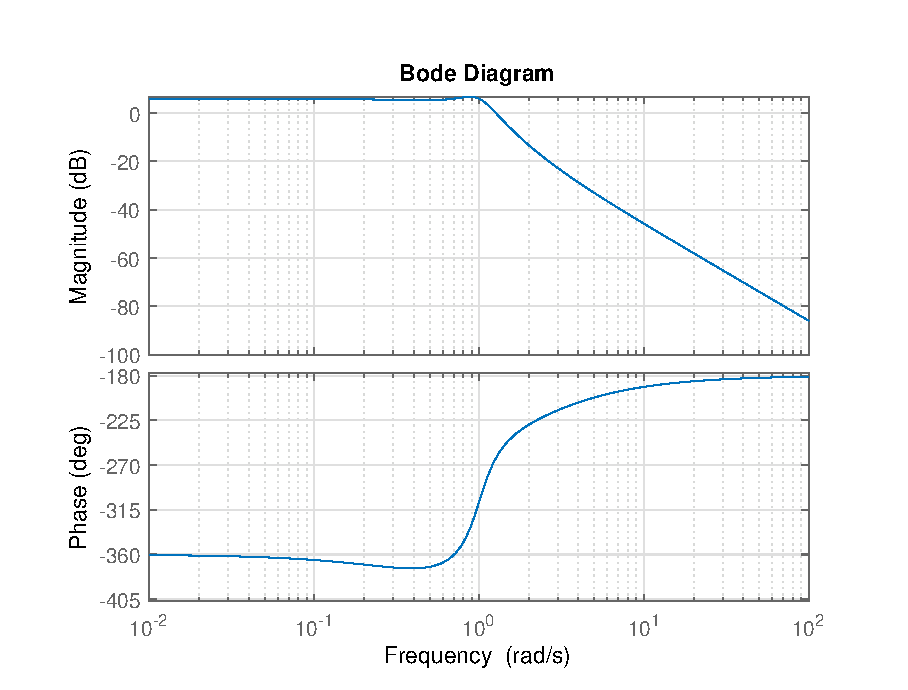
\includegraphics[width=\maxwidth{56.196688409433015em}]{figure_0.eps}
\end{center}


\begin{par}
\begin{flushleft}
In MATLAB, we can use \texttt{\textbf{margin}} to calculate the gain margin, \texttt{\textbf{Gm}}, phase margin, \texttt{\textbf{Pm}}, and associated frequencies \texttt{\textbf{Wgm}} and \texttt{\textbf{Wpm}} of SISO open-loop models. The gain and phase margin of a system \texttt{\textbf{sys}} indicates the relative stability of the closed-loop system formed by applying unit negative feedback to \texttt{\textbf{sys}}.
\end{flushleft}
\end{par}

\begin{par}
\begin{flushleft}
The gain margin is the amount of gain increase or decrease required to make the loop gain unity at the frequency \texttt{\textbf{Wgm}} where the phase angle is $-180$ (modulo $360$). In other words, the gain margin is ${{\frac{1}{g}}}$ if $g$ is the gain at the $180$ phase frequency. Similarly, the phase margin is the difference between the phase of the response and $180$ when the loop gain is 1.0. The frequency \texttt{\textbf{Wpm}} at which the magnitude is 1.0 is called the \textit{unity-gain frequency} or \textit{gain crossover frequency}.
\end{flushleft}
\end{par}

\begin{par}
\begin{flushleft}
\textbf{Note:} It is generally found that gain margins of three or more combined with phase margins between 30 and 60 degrees result in reasonable trade-offs between bandwidth and stability.
\end{flushleft}
\end{par}

\begin{par}
\begin{flushleft}
We use this function as follows: \texttt{\textbf{[Gm,Pm,Wgm,Wpm] = margin(sys)}}. \texttt{\textbf{Wgm}} is the frequency where the gain margin is measured, which is a -180 degree phase crossing frequency. \texttt{\textbf{Wpm}} is the frequency where the phase margin is measured, which is a 0dB gain crossing frequency. These frequencies are expressed in rad/s is the unit specified in the property of \texttt{\textbf{sys}}. When \texttt{\textbf{sys}} has several crossovers, \texttt{\textbf{margin}} returns the smallest gain and phase margins and corresponding frequencies. For more information about \texttt{\textbf{margin(sys)}}.
\end{flushleft}
\end{par}

\matlabheading{\textit{Question 2 (1 mark)}}

\begin{par}
\begin{flushleft}
Find the Gain Margin, Phase Margin and the corresponding frequencies for $G(s)$. (help \texttt{margin}).
\end{flushleft}
\end{par}

\begin{matlabcode}
[Gm, Pm, Wgm, Wpm] = margin(G);
\end{matlabcode}
\begin{matlaboutput}
Warning: The closed-loop system is unstable.
\end{matlaboutput}
\begin{matlabcode}

Pm
\end{matlabcode}
\begin{matlaboutput}
Pm = -82.7056
\end{matlaboutput}
\begin{matlabcode}
Gm
\end{matlabcode}
\begin{matlaboutput}
Gm = Inf
\end{matlaboutput}


\matlabheading{\textit{Question 3 (1 mark)}}

\begin{par}
\begin{flushleft}
Determine whether the open-loop system is stable or not? Based on the values of the GM and PM, What can you say about the stability of the closed-loop system? Justify your answer.
\end{flushleft}
\end{par}

\begin{matlabcode}
pole(G)
\end{matlabcode}
\begin{matlaboutput}
ans = 3x1 complex    
   0.2500 + 0.9682i
   0.2500 - 0.9682i
  -0.5000 + 0.0000i

\end{matlaboutput}
\begin{matlabcode}

% Open-loop stability
% the system has poles in the Open Right Hand Plane 
% so the open-loop system is unstable 

% Closed-loop stability
% Gm > 0 and Pm < 0 so the closed loop system is unstable
\end{matlabcode}


\matlabheading{\textit{2. Lead Compensator Design}}

\begin{par}
\begin{flushleft}
Let $G_{cl} (s)$ be the unity feedback closed-loop transfer function of $G(s)$ and could be found as follows:
\end{flushleft}
\end{par}

\begin{par}
$$G_{cl} (s)={{\frac{C_{Lead} (s)G(s)}{1+C_{Lead} (s)G(s)}}}$$
\end{par}

\begin{par}
\begin{flushleft}
A first order phase-lead compensator has the form given below:
\end{flushleft}
\end{par}

\begin{par}
$$C_{Lead} =K{{\frac{1+Ts}{1+\alpha Ts},~~\alpha <1,~~K=K_c \alpha }}$$
\end{par}

\begin{par}
\begin{flushleft}
The open-loop transfer function of the compensated system is
\end{flushleft}
\end{par}

\begin{par}
$$G_{ol} (s)=K{{\frac{1+Ts}{1+\alpha Ts}G(s)}}$$
\end{par}

\begin{par}
\begin{flushleft}
We want to design a lead compensator such that the following conditions are satisfied:
\end{flushleft}
\end{par}

\begin{itemize}
\setlength{\itemsep}{-1ex}
   \item{\begin{flushleft} Steady-state error to a step input $\le 0.05$. \end{flushleft}}
   \item{\begin{flushleft} Phase margin $\ge 45$. \end{flushleft}}
\end{itemize}

\begin{par}
\begin{flushleft}
The first step in the lead design is to provide the required static position error constant. Define $G_1 (s)$ as follows:
\end{flushleft}
\end{par}

\begin{par}
$$G_1 (s)=KG(s)$$
\end{par}

\matlabheading{\textit{Question 4 (1 mark)}}

\begin{par}
\begin{flushleft}
Find the value of $K$ such that the steady state conditions are satisfied.
\end{flushleft}
\end{par}

\begin{matlabcode}
K = 9.5 % (Caluculated)
\end{matlabcode}
\begin{matlaboutput}
K = 9.5000
\end{matlaboutput}


\begin{par}
\begin{flushleft}
With this value of $K$, the compensated system will satisfy the steady-state requirement. Now we shall plot the Bode plot of $G_1 (s)$.
\end{flushleft}
\end{par}

\matlabheading{\textit{Question 5 (1 mark)}}

\begin{par}
\begin{flushleft}
Draw the Bode plot of $G_1 (s)$ and find the GM, PM, and corresponding frequencies. (Draw the Bode plot of $G(s)$ again to see the difference)
\end{flushleft}
\end{par}

\begin{matlabcode}
% Draw the Bode plot
G1 = K * G
\end{matlabcode}
\begin{matlaboutput}
G1 =
 
     9.5 s + 19
  -----------------
  2 s^3 + 1.5 s + 1
 
Continuous-time transfer function.
\end{matlaboutput}
\begin{matlabcode}

bode(G1)
grid on
\end{matlabcode}
\begin{center}
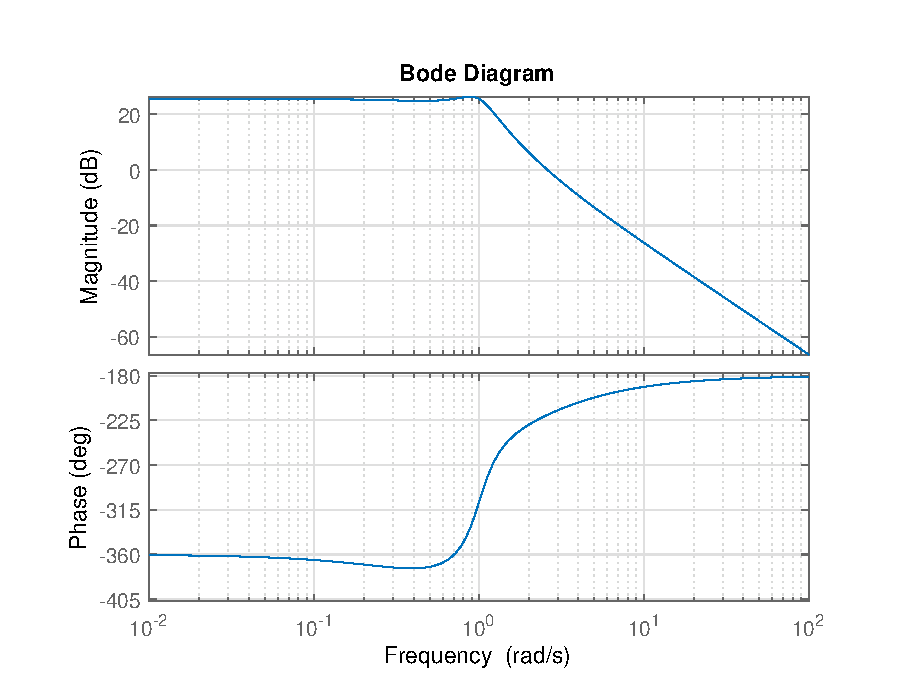
\includegraphics[width=\maxwidth{56.196688409433015em}]{figure_1.eps}
\end{center}
\begin{matlabcode}


% Determine the gain and phase margin of G1 = KG (from Bode plot)
[Gm, Pm, Wgm, Wpm] = margin(G1);
\end{matlabcode}
\begin{matlaboutput}
Warning: The closed-loop system is unstable.
\end{matlaboutput}
\begin{matlabcode}

Pm
\end{matlabcode}
\begin{matlaboutput}
Pm = -39.4443
\end{matlaboutput}
\begin{matlabcode}
Gm
\end{matlabcode}
\begin{matlaboutput}
Gm = Inf
\end{matlaboutput}


\begin{par}
\begin{flushleft}
The phase-lead compensator will add positive phase to our system over the frequency range ${{\frac{1}{aT}}}$ and ${{\frac{1}{T}}}$, which are called the corner frequencies.
\end{flushleft}
\end{par}

\matlabheading{\textit{Question 6 (2 marks)}}

\begin{par}
\begin{flushleft}
Based on the values of the GM and PM and the corresponding frequencies you found in Question 5, design the lead compensator that satisfies the conditions given in this part. Write the final lead compensator as a transfer function.
\end{flushleft}
\end{par}

\begin{par}
\begin{flushleft}
Hint: \texttt{\textbf{sin()}} in \texttt{\textbf{MATLAB}} uses radian as the input argument. For input arguments in degree use \texttt{\textbf{sind()}}.
\end{flushleft}
\end{par}

\begin{matlabcode}
% The desired phase margin is 45
PMd = 45;   

% Determine alpha
alpha = (1 - sind(PMd - Pm + 1)) / (1 + sind(PMd - Pm + 1))
\end{matlabcode}
\begin{matlaboutput}
alpha = 0.0016
\end{matlaboutput}
\begin{matlabcode}

% Determine the crossover frequency (from bode plot)
mag_cross_db = 10 * log10(alpha)
\end{matlabcode}
\begin{matlaboutput}
mag_cross_db = -28.0075
\end{matlaboutput}
\begin{matlabcode}

% from the bode plot at M = -28: 
w_cross = 11.2 
\end{matlabcode}
\begin{matlaboutput}
w_cross = 11.2000
\end{matlaboutput}
\begin{matlabcode}

% Write the final lead compensator transfer function
T = 1 / (w_cross * sqrt(alpha))
\end{matlabcode}
\begin{matlaboutput}
T = 2.2447
\end{matlaboutput}
\begin{matlabcode}

CLead = K * (1 + T * s) / (1 + alpha * T * s)
\end{matlabcode}
\begin{matlaboutput}
CLead =
 
  21.32 s + 9.5
  --------------
  0.003551 s + 1
 
Continuous-time transfer function.
\end{matlaboutput}


\matlabheading{\textit{Question 7 (1 mark)}}

\begin{par}
\begin{flushleft}
Produce the Bode diagram of the lead compensator you found in Question 6.
\end{flushleft}
\end{par}

\begin{matlabcode}
% Draw the Bode plot

bode(CLead)
grid on
\end{matlabcode}
\begin{center}
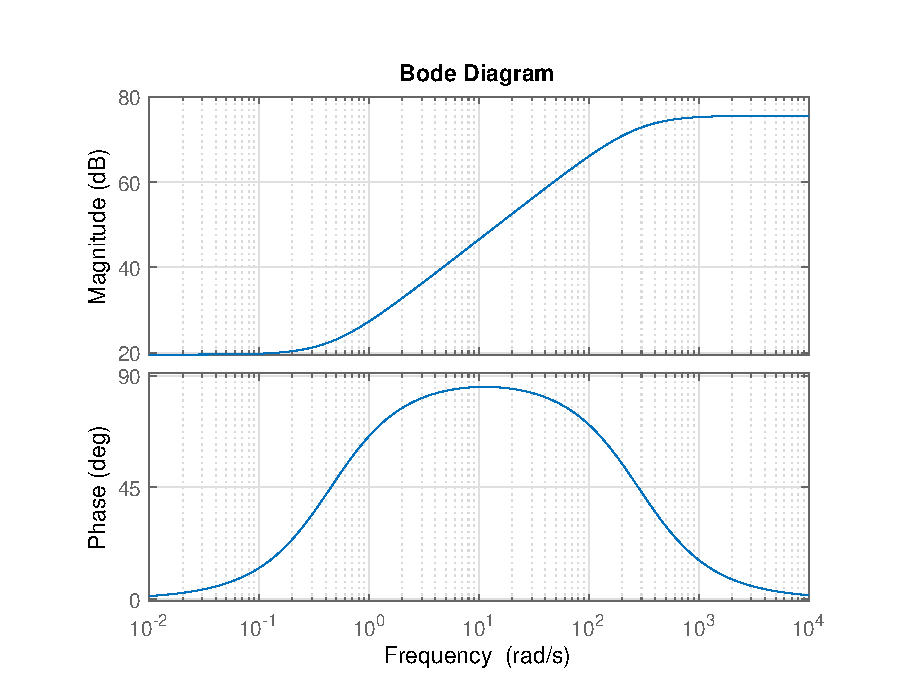
\includegraphics[width=\maxwidth{56.196688409433015em}]{figure_2.eps}
\end{center}


\matlabheading{\textit{Question 8 (1 mark)}}

\begin{par}
\begin{flushleft}
Produce the Bode diagram of the transfer function $G_{Lead} (s)=C_{Lead} (s)G(s)$. Check whether the specifications are satisfied or not (use \texttt{\textbf{margin}} to check the GM and PM).
\end{flushleft}
\end{par}

\begin{matlabcode}
% Define Gcl
GLead  = CLead * G
\end{matlabcode}
\begin{matlaboutput}
GLead =
 
              21.32 s^2 + 52.15 s + 19
  -------------------------------------------------
  0.007103 s^4 + 2 s^3 + 0.005327 s^2 + 1.504 s + 1
 
Continuous-time transfer function.
\end{matlaboutput}
\begin{matlabcode}

% Draw Bode Plot
bode(GLead)
grid on
\end{matlabcode}
\begin{center}
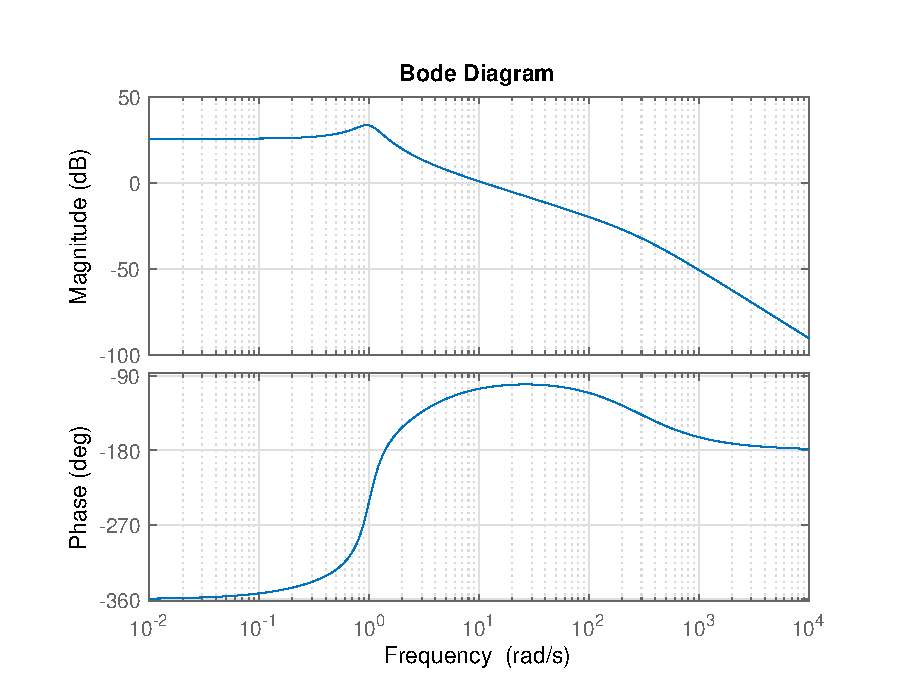
\includegraphics[width=\maxwidth{56.196688409433015em}]{figure_3.eps}
\end{center}
\begin{matlabcode}

[GmLead, PmLead, WgmLead, WpmLead] = margin(GLead);
PmLead
\end{matlabcode}
\begin{matlaboutput}
PmLead = 75.0343
\end{matlaboutput}
\begin{matlabcode}
GmLead
\end{matlabcode}
\begin{matlaboutput}
GmLead = 0.0455
\end{matlaboutput}
\begin{matlabcode}

if PmLead >= 45
    disp('The phase margin requirements are satisfied');
else
    disp(['The phase margin obtained ' num2str(PmLead) ' is less than required 45 degrees.']);
end
\end{matlabcode}
\begin{matlaboutput}
The phase margin requirements are satisfied
\end{matlaboutput}


\matlabheading{\textit{Question 9 (1 mark)}}

\begin{par}
\begin{flushleft}
Plot the step response of the closed-loop system $G_{cl} (s)$. (help \texttt{step}) .
\end{flushleft}
\end{par}

\begin{matlabcode}
Gcl = GLead / (1 + GLead)
\end{matlabcode}
\begin{matlaboutput}
Gcl =
 
                0.1515 s^6 + 43.02 s^5 + 104.5 s^4 + 70.34 s^3 + 99.83 s^2 + 80.72 s + 19
  ------------------------------------------------------------------------------------------------------
  5.045e-05 s^8 + 0.02841 s^7 + 4.152 s^6 + 43.06 s^5 + 110.6 s^4 + 74.36 s^3 + 102.1 s^2 + 83.72 s + 20
 
Continuous-time transfer function.
\end{matlaboutput}
\begin{matlabcode}

step(Gcl)
grid on
\end{matlabcode}
\begin{center}
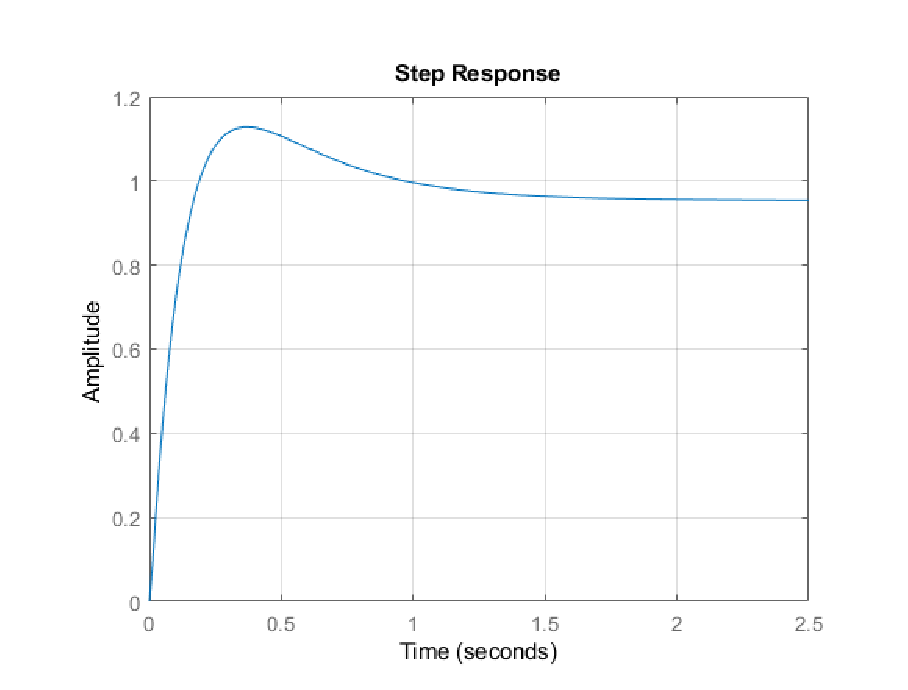
\includegraphics[width=\maxwidth{56.196688409433015em}]{figure_4.eps}
\end{center}

\end{document}
